\documentclass{article}
\usepackage[utf8]{inputenc}

\usepackage{amssymb}

\usepackage{hyperref}
\hypersetup{
    colorlinks=true,
    linkcolor=blue,
    filecolor=magenta,      
    urlcolor=cyan,
}

\usepackage{graphicx}
\usepackage{float}

\usepackage{enumitem}

\title{16.811 Project Report: Kalman Filter SLAM}
\author{Rockey Hester}
\date{December 12, 2019}

\begin{document}

\maketitle

\section{Introduction}

The Kalman Filter and its derivatives are ubiquitous techniques for state estimation, but undergraduate courses in controls and robotics commonly gloss over the details of their derivation and implementation due to the availability of many open source libraries and their difficulty of implementation. This project is an attempt to fill in some of the gaps in my knowledge by exploring the derivation and implementation of the Kalman Filter and how they can be applied to one of my favorite problems in robotics - Simultaneous Localization and Mapping (SLAM). First the Kalman Filter equations are presented and explained along with some other considerations for implementation and application to SLAM. Then, the dynamics for a particular system, the commonly used Jackal wheeled robot, are derived. Next, the Kalman Filter state estimate for a simulated Jackal robot is compared to simply integrating the equations of motion for a driving task. Lastly, SLAM is briefly explored using an existing library.

\section{Related Works}

Choset et. al derive the linear Kalman Filter, Extended Kalman Filter, and Kalman Filter SLAM in [1]. The system dynamics are formulated as

$$x(k+1) = F(k) x(k) + G(k) u(k) + v(k)$$
$$y(k) = H(k) x(k) + w(k)$$

for a linear system, where $x \epsilon R^n$ is the system state, $F \epsilon R^{n \xtimes n}$ is the system dynamics, $u \epsilon R^m$ is the input, $G \epsilon R^{n \times m}$ is the input dynamics, $v \epsilon R^n$ with covariance $V(k) \epsilon R^{n \times n}$ is the process noise, $y \epsilon R^p$ is the output, $H \epsilon R^{p \times n}$ is the sensor dynamics, $w \epsilon R^p$ with covariance $W(k) \epsilon R^{p \times p}$ is the measurement noise, and $k \epsilon Z^+$ is the time step.

The Kalman Filter is a two step process. First, the current state, the system dynamics, and the commands to the system are used to \textit{predict} the next state (or rather, a distribution over the next state with mean $\hat{x}$ and covariance $P$). Second, the prediction is \textit{updated} using the sensor data by weighting the innovation $\nu$ (the difference between the actual measurement and the measurement we would expect to receive from the predicted state) with the reliability of the sensors.

The prediction equation is as follows:

$$\hat{x}(k+1|k) = F(k)\hat{x}(k|k) + G(k) u(k)$$
$$P(k+1|k) = F(k) P(k|k) F(k)^T + V(k)$$

The update equation is as follows:

$$\hat{x}(k+1|k+1) = \hat{x}(k+1|k) + R\nu$$
$$P(k+1|k+1) = P(k+1|k) - RH(k+1) P(k+1|k)$$

where

$$\nu = y(k+1) - H(k+1) x(k+1|k)$$
$$S = H(k+1) P(k+1|k) H(k+1)^T + W(k+1)$$
$$R = P(k+1|k) H(k+1)^T S^{-1}$$

The Extended Kalman Filter (EKF) is a modified version of the linear Kalman Filter that accounts for systems with nonlinear dynamics (which means that they're unable to be formulated into the matrices $F$, $G$, and $H$).

The new system dynamics are defined as

$$x(k+1) = f(x(k), u(k), k) + v(k)$$
$$y(k) = h(x(k), k) + w(k)$$

where all is the same as before except $f$ is a function mapping the state and input to $R^n$ and $h$ is a function mapping the state to $R^p$. All that must be done to get these equations into a usable form is to linearize $f$ and $h$.

The prediction equations are then

$$\hat{x}(k+1|k) = f(\hat{x}(k|k), u(k), k)$$
$$P(k+1|k) = F(k) P(k|k) F(k)^T + V(k)$$

where

$$F(k) = \frac{\partial f}{\partial x}\Big|_{x=\hat{x}(k|k)} = \pmatrix{
\frac{\partial f_1}{\partial x_1} & \frac{\partial f_1}{\partial x_2} & \dots & \frac{\partial f_1}{\partial x_n} \cr 
\frac{\partial f_2}{\partial x_1} & \frac{\partial f_2}{\partial x_2} & \dots & \frac{\partial f_2}{\partial x_n} \cr
\vdots & \vdots & \ddots & \vdots \cr
\frac{\partial f_n}{\partial x_1} & \frac{\partial f_n}{\partial x_2} & \dots & \frac{\partial f_n}{\partial x_n}}_{x=\hat{x}(k|k)}$$

The update is exactly the same as before except

$$H(k+1) = \frac{\partial h}{\partial x}\Big|_{x = \hat{x}(k+1|k)} = \pmatrix{
\frac{\partial h_1}{\partial x_1} & \frac{\partial h_1}{\partial x_2} & \dots & \frac{\partial h_1}{\partial x_n} \cr 
\frac{\partial h_2}{\partial x_1} & \frac{\partial h_2}{\partial x_2} & \dots & \frac{\partial h_2}{\partial x_n} \cr
\vdots & \vdots & \ddots & \vdots \cr
\frac{\partial h_n}{\partial x_1} & \frac{\partial h_n}{\partial x_2} & \dots & \frac{\partial h_n}{\partial x_n}}_{x=\hat{x}(k+1|k)}$$

The Kalman Filter can be extended to solve the problem of SLAM by estimating the locations of both the robot and any landmarks detected in the environment at the same time. This can be done by extending the state $x$ to include the positions of the landmarks on top of the regular state of the robot and by extending the sensor model to include some measure of the relative positions of the robot and each landmark (such as range and bearing via laser scan) as well as the other sensors on the robot (e.g. IMU, wheel odometry, etc). After linearizing any nonlinear dynamics, the prediction and update equations are exactly the same as in the Kalman Filter and EKF.

The new state $x$ can be represented as

$$x = \pmatrix{\textbf{x_r} & x_{l1} & y_{l1} & x_{l2} & y_{l2} & \dots & x_{ln} & y_{ln}}^T$$

Since the landmarks are assumed to be fixed, the covariance $V(k)$ is just

$$V(k) = \pmatrix{
V_r(k) & 0 & \dots & 0 \cr 
0 & 0 & \dots & 0 \cr
\vdots & \vdots & \ddots & \vdots \cr
0 & 0 & \dots & 0}$$

where $V_r(k)$ is the covariance of the process noise of just the robot. The landmarks have no process noise.

One relative position measurement is the following range and bearing model, which measures the distance and angle from the robot to each landmark $l_i$. 

$$y_i(k) = \pmatrix{\sqrt{(x_{li}(k)-x_r(k))^2 + (y_{li}(k)-y_r(k))^2}\cr
\texttt{atan2}{(y_{li}(k)-y_r(k)), (x_{li}(k)-x_r(k))}} + w_i(k)$$

The covariance $W(k)$ can be thought of as before since even though the landmarks are fixed, there is still noise in measuring their locations.

The final consideration for Kalman Filter SLAM is the problem of \textit{data association} - it is not immediately clear which landmark each measurement is associated with. This problem can be solved with the Mahalanobis distance $\chi$.

$$\chi_{ij}^2 = \nu_{ij} S_{ij}^{-1} \nu_{ij}^T$$

$$\chi_{ij}^2 = (y(k)_i-h(k)_j)^T S_{ij}^{-1} (y(k)_i-h(k)_j)$$

The Mahalanobis distance is computed for every pair of measurements and possible landmarks. Generally, a measurement is associated with the landmark with the lowest corresponding Mahalanobis distance. However, if there is no landmark with a sufficiently low Mahalanobis distance, this indicates that a new landmark should be initialized and added to the state.

In his lecture on the Kalman Filter [2], Simon explains the process of computing $V(k)$ and $W(k)$ for a given system. This can be done by fitting a distribution to the system output from zero input over time.

The derivation of Kalman Filter SLAM assumes that the positions of the landmarks can be measured directly. However, for many commonly used sensors such as LiDAR, this is not the case. Landmark positions must be extracted from the raw point cloud data. This is done using techniques such as FLIRT and FALKO [3] and is very similarl to the process of finding keypoints and computing descriptors for images.

The Jackal robot from Clearpath Robotics [4] is a popular wheeled robot for research. It is accompanied by a simulator in ROS Gazebo and RViz, which can accommodate multiple sensors, including IMU, wheel odometry, and LiDAR.

As a baseline for the performance of a working SLAM system, the ROS gmapping library is used with the aforementioned Jackal simulator. Gmapping is based on the particle filter [5] rather than the Kalman Filter.


\section{Approach}

The Jackal simulator in ROS Gazebo is used with data visualization in RViz. The system state consists of the position and orientation of the robot in the 2D plane, the inputs to the system are the linear and angular velocity $v$ and $\omega$, and the outputs are only.

$$f(x) = \pmatrix{\cos{\theta(k)}v(k) + x(k) \cr
                  \sin{\theta(k)}v(k) + y(k) \cr
                  v(k) \cr
                  \omega(k) + \theta(k) \cr
                  \omega(k)}$$
$$F(x) = \pmatrix{1 & 0 & \cos{theta(k)} & -\sin{theta(k)}v(k) & 0 \cr
                  0 & 1 & \sin{theta(k)} & \cos{theta(k)}v(k) & 0 \cr
                  0 & 0 & 1 & 0 & 0 \cr
                  0 & 0 & 0 & 1 & 0 \cr
                  0 & 0 & 0 & 0 & 1}$$
$$h(x) = \pmatrix{v(k) \cr \omega(k)}$$
$$H(x) = \pmatrix{0 & 0 & 1 & 0 & 0 \cr 0 & 0 & 0 & 0 & 1}$$

- noise covariance matrix determination

TODO

\begin{figure}[!htb]
\minipage{0.48\textwidth}
  \includegraphics[width=\linewidth]{v_noise.png}
  \caption{}
\endminipage\hfill
\minipage{0.48\textwidth}
  \includegraphics[width=\linewidth]{omega_noise.png}
  \caption{}
\endminipage
\end{figure}

$$W(k) = \pmatrix{0.00001 & 0 \cr 0 & 0.01}$$

\begin{figure}[!htb]
\minipage{0.32\textwidth}
  \includegraphics[width=\linewidth]{x_high_noise.png}
  \caption{}
\endminipage\hfill
\minipage{0.32\textwidth}
  \includegraphics[width=\linewidth]{y_high_noise.png}
  \caption{}
\endminipage\hfill
\minipage{0.32\textwidth}%
  \includegraphics[width=\linewidth]{theta_high_noise.png}
  \caption{}
\endminipage
\end{figure}

$$V(k) = \pmatrix{0.00001 & 0 & 0 & 0 & 0 \cr
                  0 & 0.00001 & 0 & 0 & 0 \cr
                  0 & 0 & 0.00001 & 0 & 0 \cr
                  0 & 0 & 0 & 0.00001 & 0 \cr
                  0 & 0 & 0 & 0 & 0.00001}$$

- compare kalman filter to integration of equations of motion (equivalent to calling $f$ over and over)

TODO

- gmapping baseline (talk about gazebo simulator and Rviz)

TODO


\section{Results}

- kalman filter performance (graphs of estimate vs actual over time, comparison to just integrating equations of motion)

TODO

\begin{figure}[!htb]
\minipage{0.32\textwidth}
  \includegraphics[width=\linewidth]{x_comparison.png}
  \caption{}
\endminipage\hfill
\minipage{0.32\textwidth}
  \includegraphics[width=\linewidth]{y_comparison.png}
  \caption{}
\endminipage\hfill
\minipage{0.32\textwidth}%
  \includegraphics[width=\linewidth]{theta_comparison.png}
  \caption{}
\endminipage
\end{figure}

- map produced by gmapping

TODO

\begin{figure}[!htb]
\minipage{0.48\textwidth}
  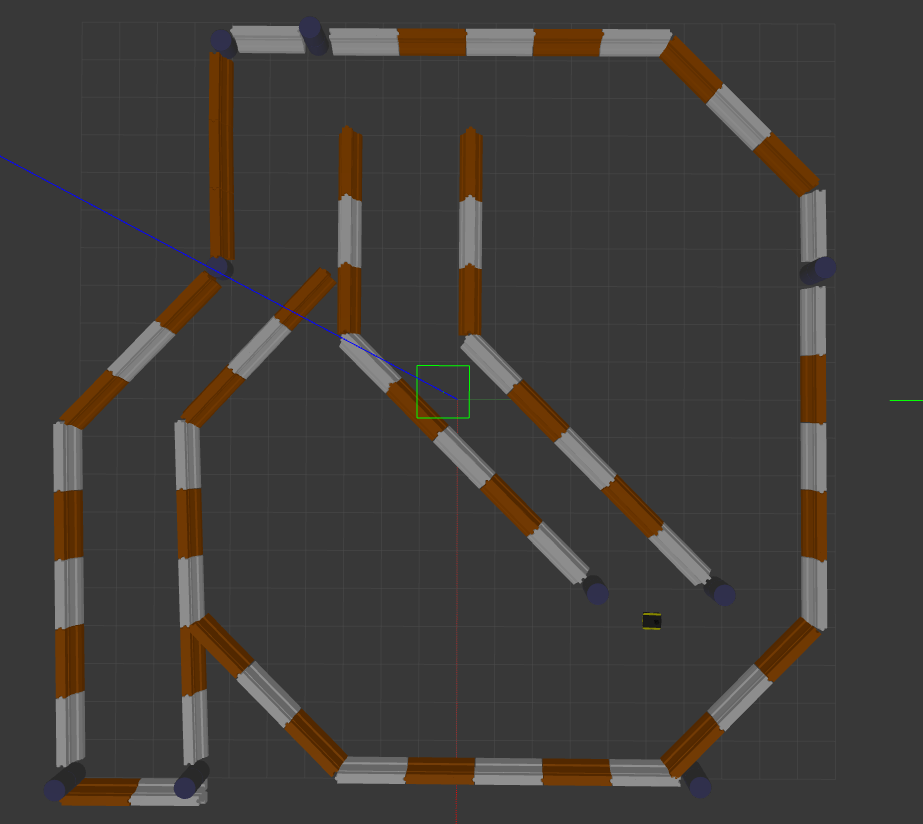
\includegraphics[width=\linewidth]{actual_map.png}
  \caption{}
\endminipage\hfill
\minipage{0.48\textwidth}
  \includegraphics[width=\linewidth]{slam_progress.png}
  \caption{}
\endminipage
\end{figure}

\section{Discussion}

- kalman filter performance (dependent on noise covariances)

TODO

- gmapping performance

TODO

- future

TODO (never implement kalman filter again but would like to do SLAM)

\section*{References}

\begin{enumerate}
    \item H. Choset, K. Lynch, S. Hutchinson, G. Kantor, W. Burgard, L. Kavraki, S. Thrun, "Principles of Robot Motion", MIT Press, ch. 8, pp. 289-319, 2016, isbn: 9780262303958
    
    \item D. Simon, "A Crash Course on Kalman Filtering", Cleveland State University, 2014
    
    \item F. Kallasi, D. L. Rizzini and S. Caselli, "Fast Keypoint Features From Laser Scanner for Robot Localization and Mapping," in IEEE Robotics and Automation Letters, vol. 1, no. 1, pp. 176-183, Jan. 2016.
doi: 10.1109/LRA.2016.2517210

    \item Clearpath Robotics, "Jackal Simulator", 2015
    
    \item G. Grisetti, C. Stachniss and W. Burgard, "Improved Techniques for Grid Mapping With Rao-Blackwellized Particle Filters," in IEEE Transactions on Robotics, vol. 23, no. 1, pp. 34-46, Feb. 2007.
doi: 10.1109/TRO.2006.889486
\end{enumerate}

\end{document}